\chapter{显微成像系统整体方案设计}
本显微成像检测系统由光学模块、图像处理模块、图像采集模块、图像归档显示模块等构成。在整体设计流程中,关键的技术包括图像传感器的分析与选择、图像主处理器及预处理器的选择等。本章在光学基础上,根据需求和情境重点分析了各个不同模块需要的硬件优势方面和选型,并对此进行较为详细的讲述。可见的一个分类的图示如:
(画图,,数据流生成方面流程)

\section{显微基本原理}
\subsection{光学成像原理}

显微镜的成像如图\ref{fig:micro_1}所示,小物体AB在物镜的焦距之外,人眼在另一边的距离除观察,AB形成放大倒立的实像A'B',而这一实像正好在目镜的焦距以内的附近处,再一次经过目镜放大之后,在明视距离d处形成正立虚像A"B"。
\begin{figure}[h]
	\centering
	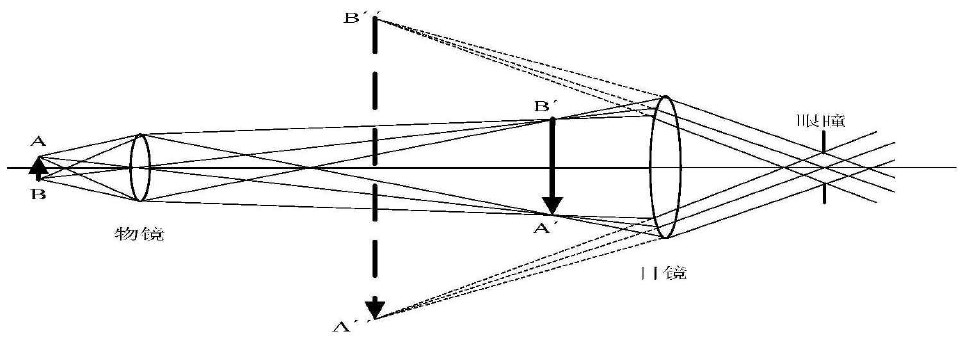
\includegraphics[width=0.7\linewidth]{Figure/micro_1}
	\caption[显微镜成像光路图]{显微镜成像光路图}
	%\caption{显微镜成像光路图}
	\label{fig:micro_1}
\end{figure}

显微镜的视觉放大率定义为:

\begin{figure}[h]
\centering
\label{j2}
	$J = l_{0}\cdot d / f_{1}f_{2}$
\end{figure}
式\ref{j2}中$d$ 是明视距离,$1_{0}$为物镜到目镜的距离,$f_{1}$为物镜的焦距,$f_{2}$为目镜的焦距。此处的角放大率为物镜的线放大率和目镜的角放大率的乘积。
数值孔径的孔径角的正弦与透镜和物体之间介质的折射率的乘积,而显微镜的分辨率与光的波长和物镜的数值孔径有关,波长越短,数值孔径越大,分辨率越大。


\subsection{显微镜结构构造}
普通光学显微镜的构造可分为两部分:一为机械装置,二为光学系统 。机械装置由镜座、镜筒、物镜转换器、载物台、推动器、粗动螺旋和微动螺旋等部件组成。光学系统由目镜、物镜、聚光器、光源、滤光片、虹彩光圈等组成。

物镜是决定显微镜性能的最重要部件,安装在物镜转换器上,接近被观察的物体,故叫做物镜或接物镜。通常目镜由上下两组透镜组成,上面的透镜叫做接目透镜,下面的透镜叫做会聚透镜或场镜。聚光器也叫集光器。位于标本下方的聚光器支架上。它主要由聚光镜和可变光阑组成。其中,聚光镜可分为明视场聚光镜和暗视场聚光镜。反光镜是一个可以随意转动的双面镜,直径为50mm,一面为平面,一面为凹面,其作用是将从任何方向射来的光线经通光孔反射。平面镜上反射光线的能力较弱,适合在光线较强时使用,凹面镜反射光线的能力较强,适合在光线较弱时使用。
	 
\section{显微成像处理平台器件选型}
\subsection{显微镜头物镜目镜选型(不开工)}
(1)显微物镜的设计 在本系统设计中,对测量精度要求较高,要求系统分辨本领达到 0.5m。本显微成 像系统的分辨率由光学镜头的分辨率和 CMOS 摄像头的分辨率共同决定。系统中光学 镜头部分对物体进行放大,先考虑光学系统的分辨率:
上式中, n 为物空间介质折射率,为照明光源的中心波长,是系统的分辨率,因 此在照明波长确定时,只能增大镜头的数值孔径来提升分辨率。 整个系统光学放大率由系统要求的分辨率大小和CMOS的像元尺寸决定,如下式,
式中,是系统中 CMOS 芯片的最小可分辨尺寸,为系统的分辨率,为系统总的放 大率。 根据上述的设计分析,选用了消色差物镜中放大倍数中等的李斯特物镜。它的结 构采用两个分离的双胶组合透镜组,垂轴放大率达到 10 倍,数值孔径(NA)设计值 为 0.61。李斯特型物镜的设计原则包括:(一)各个双胶合透镜组具有相同的偏角,后 组比前组的偏角略大。(二)光阑位置处于第一个双胶合透镜处。采用两组双胶合透镜 来抵消球差和慧差,物镜的总焦距就等于两组双胶合透镜之间的距离。前一个双胶合 组的焦距两倍于物镜焦距。物镜的总焦距与第二个双胶合组焦距相同。(三)采取两个 双胶合透镜分别单独校正系统的球差、慧差和色差,这种设计的优点是采用两个双胶 合透镜组合,组合在一起为一个中倍显微物镜,移去一个双胶合组后可作为低倍显微 物镜[28]。 按照物镜设计要求:物镜要求放大倍数为 10 倍,系统光源照明采用中心波长为 550nm 的光源,由式 NA=nsinu 计算可得,透镜数值孔径大小为 0.61,通过以上几个参 数的确定,选出符合参数要求的镜片组合。选定透镜组合后采用 ZEMAX 对设计进行 仿真,对光线进行追迹、计算像差,对设计不满意的参数,再次重新选择玻璃材料, 重复上面的仿真计算[29],直到达到设计要求。
\subsection{图像传感器的选型}
\subsubsection{CMOS和CCD的比较}
固体图像传感器已经广泛地应用于生活各处,包括像电子照相机、DV、智能监控、手机、平板和摄像头等。固体图像传感器是利用半导体材料的内光电效应原理制成的光电转换器件,依据工艺结构可以分为两大类:一类是电荷耦合器件(CCD)图像传感器;另一类是互补金属氧化物(CMOS)图像传感器。两种目前常见的图像传感器都是上世纪60年代开始研制,在当时由于CCD图像传感器灵敏度更高、噪声较低而成为当时图像传感器的主流。而CMOS图像传感器由于工艺上的提升限制,长时间未能摆脱光照灵敏度低、噪声无法下降和图像分辨率低等不足。于此同时,CCD图像传感器由于敏感元件和信号处理电路无法集成在同一芯片上,使得照相机体积大、功耗大。

进入新世纪,时间发展,随着互联网向移动互联网的转移,智能手机的发展十分迅速,由于CMOS图像传感器却有集成度高、体积小、功耗小和造价低等优点,十分适合在手机上进行集成,考虑到两种图像传感器的技术特点和缺点改进方式,随集成电路设计技术和迭代工艺水平的提高,CMOS图像传感器过去存在的缺点,现在开始逐渐进行技术攻关,常见的背照式结构给CMOS图像传感器在光线摄入上有长足的发展,而且它其固有的特点更是CCD器件所无法比拟的,因而它再次成为研究和工业需求的热点。

CCD和CMOS两者在多个维度上有着较大特性上的差异:

1.系统集成 \\
CMOS图像传感器易于在SoC上集成,便于在同一芯片中同时进行内部的信号降噪、数据整合和数据处理,片上数据传输率高,与周边电路的整合性高,更可可将与信号处理器整合在一起,如图所示,便于大幅度减小对应模块的主板面积占用。由于CCD和CMOS两者采用不同的制造工艺,所以CCD难以装入SoC。因此,一般认为CMOS图像传感器可以广泛使用在各个嵌入式领域。

2.性能特性\\
在实际应用方面,性能特性是进行芯片选型取舍的极为重要的因素。CMOS图像传感器由于多个放大器的存在,不同一组生产的放大器放大情况有细微差异,导致最终的图像输出噪声较多。此外,由于集成度高的缘故,各元件、电路之间距离较近,相互之间的光、电、磁干扰显得严重,噪声对图像质量影响很大。在需要的电源数方面,相对于CCD图像传感器需要三或四组电源,CMOS图像传感器则只需一个即可。此外CMOS图像传感器利用3.3V电源即可驱动,相比之下电源消耗量比CCD图像传感器低。因此,在功耗和电压方面,CMOS图像传感器比CCD图像传感器在小型化嵌入式设备中有更大的优势。此外,CMOS信号读取的方式较为简易,电路设计相应也可简单。

3.可靠性\\
两种图像传感器在商用及工业应用领域具有等价的可靠性。在极端恶劣的应用环境中,由于CMOS图像传感器充分提高系统集成度、降低模块间耦合,借助设计良好的封装和焊接技术,其可靠性优于CCD图像传感器。

(列表添加图示和相关内容):
%\caption{CCD和CMOS特性比较}\label{Tab:cmos1}	
\begin{table}[ht]
	
\begin{tabular}{|L{2.2cm}|C{4cm}|R{4cm}|}
\toprule[1pt]
\hline
	& CMOS图像传感器 & CCD图像传感器 \\ \hline
	感光灵敏度 & 低 & 高 \\ \hline
	噪声电子数 & 200 & 50 \\ \hline
	电路集成度 & 高 & 低 \\ \hline
	工艺难度 & 小 & 大 \\ \hline
	成本 & 低 & 高 \\ \hline
	功耗 & 低 & 高 \\  \hline
\end{tabular} 
\end{table}

\subsubsection{图像传感器的选择}
在图像传感器的选择上,需要考虑成像质量,分辨率,集成度,接口匹配,适配度等几项重要指标。由上面的比较可以知道,CMOS图像传感器的集成度远
远优于CCD图像传感器。CMOS图像传感器可将多个处理器,控制器模块集成到一块芯片上,
直接输出数字信号,减小开发难度。而在成向质量,分辨率上,两者均能达到要求,最关注的集成性,低功耗,采样速度高等特点,CMOS图像传感器占有很大的优势,在考虑到成本问题之后,决定选用CMOS传感器作为图像采集的模块。
这里经过多次比对,决定选择SONY的IMX系列传感器。SONY最近数年在CMOS技术上的大幅度改进使得CMOS传感器的图片质量开始接近数码相机的质量。尤其是背照式技术和堆栈式技术的使用,让CMOS图像传感器进一步接近CCD图像传感器的功能。
在IMX系列中,由一张图表看出不同型号的特点,进行比较分析。图放在这里看参数比对。。。
\begin{figure}[h]
\centering
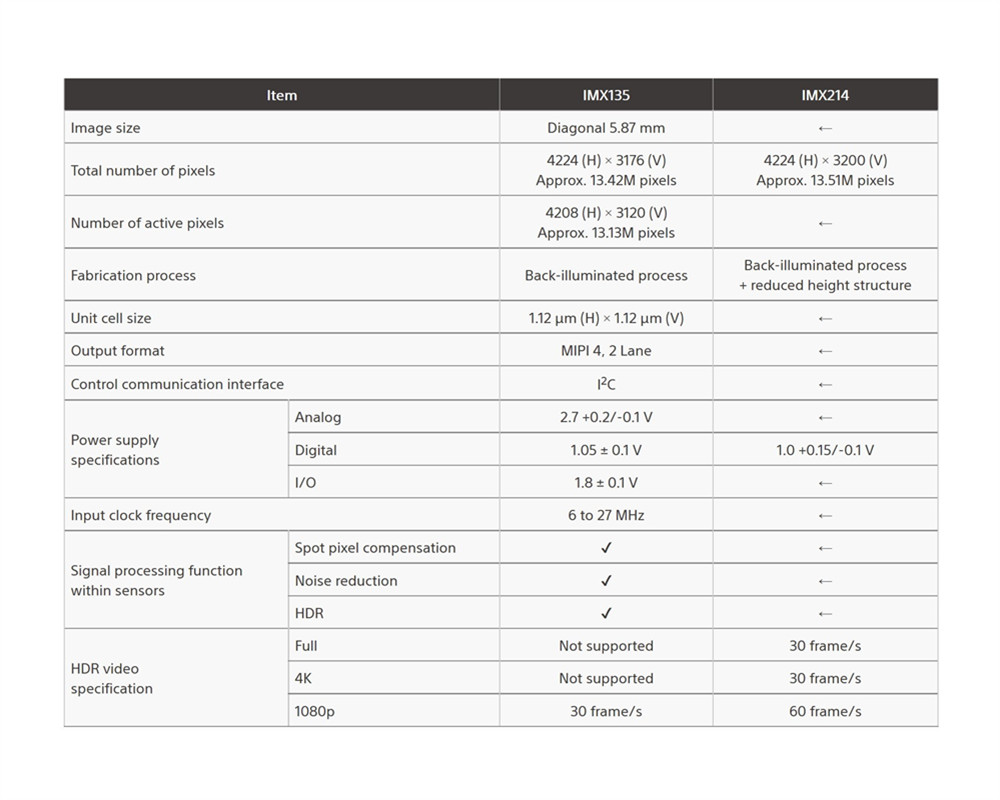
\includegraphics[width=0.7\linewidth]{Figure/IMXCMOSp}
\caption{什么135214的图}
\label{fig:IMXCMOSp}
\end{figure}


\subsection{图像处理方案研究}
实时图像处理系统要求系统需要在有限的时间内完成大量数据的运算。可尝试实现的实现有下面几种:基于PC的数据处理,基于DSP的数字信号处理,基于ARM的通用事务处理。
(1)在PC上的数据处理:是常见的图像处理方式,利用高级编程语言进行算法编程,但在实时图像数据处理上可能需要占用CPU大量的浮点计算能力,然而CPU更适合进行整数计算,在PC中大量的浮点运算通常放在GPU中运行。
(2)基于DSP的数字信号处理:通用可编程的DSP在嵌入式领域中有数字信号处理精度高,速度快,一定的编程性等优势,相对而言算法较为复杂,在高速图像处理中一定优势。
(3)基于ARM的数据处理:随着VLSI技术的不断进步,ARM在近年来在嵌入式领域上的使用比率逐渐上升,市场上借助手机的快速发展ARM的出货量和迭代速度变更极快。此外,ARM有比较强的事物管理功能,可利用通用的语言和驱动,也可方便设计图形界面和应用程序。(ARM下的Cortex-M0 处理器 ras的zero0)
)

下面表将三者的情况作出下面的对比。(后面更新)

\begin{table}[ht]
	
	\begin{tabular}{|L{2.2cm}|C{4cm}|R{4cm}|}
		\toprule[1pt]
		\hline
		& CMOS图像传感器 & CCD图像传感器 \\ \hline
		感光灵敏度 & 低 & 高 \\ \hline
		噪声电子数 & 200 & 50 \\ \hline
		电路集成度 & 高 & 低 \\ \hline
		工艺难度 & 小 & 大 \\ \hline
		成本 & 低 & 高 \\ \hline
		功耗 & 低 & 高 \\  \hline
	\end{tabular} 
\end{table}

综合上述因素,,
sdsdfsdfsdfsfsdf,选择树莓派作为系统处理平台,,,,,,,,,,,,,,,,
%区别是什么?:ARM具有比较强的事务管理功能,可以用来跑界面以及应用程序等,其优势主要体现在控制方面,而DSP主要是用来计算的,比如进行加密解密、调制解调等,优势是强大的数据处理能力和较高的运行速度。FPGA可以用VHDL或verilogHDL来编程,灵活性强,由于能够进行编程、除错、再编程和重复操作,因此可以充分地进行设计开发和验证。当电路有少量改动时,更能显示出FPGA的优势,其现场编程能力可以延长产品在市场上的寿命,而这种能力可以用来进行系统升级或除错。


\subsection{数据传输接口介绍(CSI USB Ethernet)}

\begin{figure}[h]
	\centering
	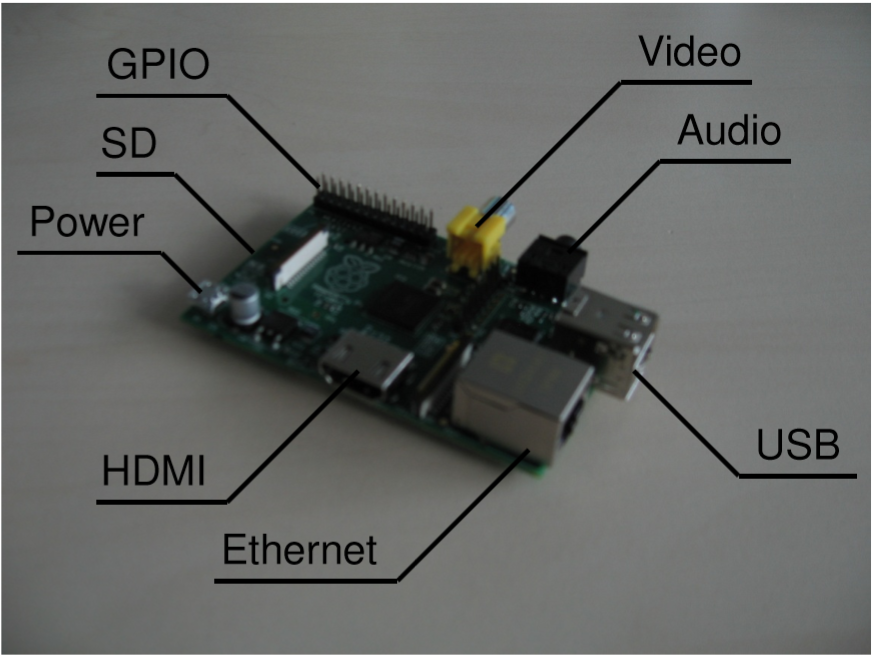
\includegraphics[width=0.7\linewidth]{Figure/rasp_1}
	\caption{树莓派基本接口}
	\label{fig:rasp_1}
\end{figure}


\section{系统平台鬼鬼鬼鬼鬼}